\documentclass[]{book}
\usepackage{lmodern}
\usepackage{amssymb,amsmath}
\usepackage{ifxetex,ifluatex}
\usepackage{fixltx2e} % provides \textsubscript
\ifnum 0\ifxetex 1\fi\ifluatex 1\fi=0 % if pdftex
  \usepackage[T1]{fontenc}
  \usepackage[utf8]{inputenc}
\else % if luatex or xelatex
  \ifxetex
    \usepackage{mathspec}
  \else
    \usepackage{fontspec}
  \fi
  \defaultfontfeatures{Ligatures=TeX,Scale=MatchLowercase}
\fi
% use upquote if available, for straight quotes in verbatim environments
\IfFileExists{upquote.sty}{\usepackage{upquote}}{}
% use microtype if available
\IfFileExists{microtype.sty}{%
\usepackage{microtype}
\UseMicrotypeSet[protrusion]{basicmath} % disable protrusion for tt fonts
}{}
\usepackage[margin=1in]{geometry}
\usepackage{hyperref}
\hypersetup{unicode=true,
            pdfborder={0 0 0},
            breaklinks=true}
\urlstyle{same}  % don't use monospace font for urls
\usepackage{natbib}
\bibliographystyle{plainnat}
\usepackage{color}
\usepackage{fancyvrb}
\newcommand{\VerbBar}{|}
\newcommand{\VERB}{\Verb[commandchars=\\\{\}]}
\DefineVerbatimEnvironment{Highlighting}{Verbatim}{commandchars=\\\{\}}
% Add ',fontsize=\small' for more characters per line
\usepackage{framed}
\definecolor{shadecolor}{RGB}{248,248,248}
\newenvironment{Shaded}{\begin{snugshade}}{\end{snugshade}}
\newcommand{\KeywordTok}[1]{\textcolor[rgb]{0.13,0.29,0.53}{\textbf{#1}}}
\newcommand{\DataTypeTok}[1]{\textcolor[rgb]{0.13,0.29,0.53}{#1}}
\newcommand{\DecValTok}[1]{\textcolor[rgb]{0.00,0.00,0.81}{#1}}
\newcommand{\BaseNTok}[1]{\textcolor[rgb]{0.00,0.00,0.81}{#1}}
\newcommand{\FloatTok}[1]{\textcolor[rgb]{0.00,0.00,0.81}{#1}}
\newcommand{\ConstantTok}[1]{\textcolor[rgb]{0.00,0.00,0.00}{#1}}
\newcommand{\CharTok}[1]{\textcolor[rgb]{0.31,0.60,0.02}{#1}}
\newcommand{\SpecialCharTok}[1]{\textcolor[rgb]{0.00,0.00,0.00}{#1}}
\newcommand{\StringTok}[1]{\textcolor[rgb]{0.31,0.60,0.02}{#1}}
\newcommand{\VerbatimStringTok}[1]{\textcolor[rgb]{0.31,0.60,0.02}{#1}}
\newcommand{\SpecialStringTok}[1]{\textcolor[rgb]{0.31,0.60,0.02}{#1}}
\newcommand{\ImportTok}[1]{#1}
\newcommand{\CommentTok}[1]{\textcolor[rgb]{0.56,0.35,0.01}{\textit{#1}}}
\newcommand{\DocumentationTok}[1]{\textcolor[rgb]{0.56,0.35,0.01}{\textbf{\textit{#1}}}}
\newcommand{\AnnotationTok}[1]{\textcolor[rgb]{0.56,0.35,0.01}{\textbf{\textit{#1}}}}
\newcommand{\CommentVarTok}[1]{\textcolor[rgb]{0.56,0.35,0.01}{\textbf{\textit{#1}}}}
\newcommand{\OtherTok}[1]{\textcolor[rgb]{0.56,0.35,0.01}{#1}}
\newcommand{\FunctionTok}[1]{\textcolor[rgb]{0.00,0.00,0.00}{#1}}
\newcommand{\VariableTok}[1]{\textcolor[rgb]{0.00,0.00,0.00}{#1}}
\newcommand{\ControlFlowTok}[1]{\textcolor[rgb]{0.13,0.29,0.53}{\textbf{#1}}}
\newcommand{\OperatorTok}[1]{\textcolor[rgb]{0.81,0.36,0.00}{\textbf{#1}}}
\newcommand{\BuiltInTok}[1]{#1}
\newcommand{\ExtensionTok}[1]{#1}
\newcommand{\PreprocessorTok}[1]{\textcolor[rgb]{0.56,0.35,0.01}{\textit{#1}}}
\newcommand{\AttributeTok}[1]{\textcolor[rgb]{0.77,0.63,0.00}{#1}}
\newcommand{\RegionMarkerTok}[1]{#1}
\newcommand{\InformationTok}[1]{\textcolor[rgb]{0.56,0.35,0.01}{\textbf{\textit{#1}}}}
\newcommand{\WarningTok}[1]{\textcolor[rgb]{0.56,0.35,0.01}{\textbf{\textit{#1}}}}
\newcommand{\AlertTok}[1]{\textcolor[rgb]{0.94,0.16,0.16}{#1}}
\newcommand{\ErrorTok}[1]{\textcolor[rgb]{0.64,0.00,0.00}{\textbf{#1}}}
\newcommand{\NormalTok}[1]{#1}
\usepackage{longtable,booktabs}
\usepackage{graphicx,grffile}
\makeatletter
\def\maxwidth{\ifdim\Gin@nat@width>\linewidth\linewidth\else\Gin@nat@width\fi}
\def\maxheight{\ifdim\Gin@nat@height>\textheight\textheight\else\Gin@nat@height\fi}
\makeatother
% Scale images if necessary, so that they will not overflow the page
% margins by default, and it is still possible to overwrite the defaults
% using explicit options in \includegraphics[width, height, ...]{}
\setkeys{Gin}{width=\maxwidth,height=\maxheight,keepaspectratio}
\IfFileExists{parskip.sty}{%
\usepackage{parskip}
}{% else
\setlength{\parindent}{0pt}
\setlength{\parskip}{6pt plus 2pt minus 1pt}
}
\setlength{\emergencystretch}{3em}  % prevent overfull lines
\providecommand{\tightlist}{%
  \setlength{\itemsep}{0pt}\setlength{\parskip}{0pt}}
\setcounter{secnumdepth}{5}
% Redefines (sub)paragraphs to behave more like sections
\ifx\paragraph\undefined\else
\let\oldparagraph\paragraph
\renewcommand{\paragraph}[1]{\oldparagraph{#1}\mbox{}}
\fi
\ifx\subparagraph\undefined\else
\let\oldsubparagraph\subparagraph
\renewcommand{\subparagraph}[1]{\oldsubparagraph{#1}\mbox{}}
\fi

%%% Use protect on footnotes to avoid problems with footnotes in titles
\let\rmarkdownfootnote\footnote%
\def\footnote{\protect\rmarkdownfootnote}

%%% Change title format to be more compact
\usepackage{titling}

% Create subtitle command for use in maketitle
\newcommand{\subtitle}[1]{
  \posttitle{
    \begin{center}\large#1\end{center}
    }
}

\setlength{\droptitle}{-2em}
  \title{}
  \pretitle{\vspace{\droptitle}}
  \posttitle{}
  \author{}
  \preauthor{}\postauthor{}
  \date{}
  \predate{}\postdate{}

% \defaultfontfeatures{
%     Path = /home/ghassany/texmf/fonts/opentype/public/fontawesome/}
\usepackage{fontawesome}

\usepackage{booktabs}
\usepackage{longtable}
\usepackage{framed,color}
\usepackage{float}
\let\origfigure\figure
\let\endorigfigure\endfigure
\renewenvironment{figure}[1][2] {
    \expandafter\origfigure\expandafter[H]
} {
    \endorigfigure
}

\definecolor{shadecolor}{RGB}{248,248,248}

\ifxetex
  \usepackage{letltxmacro}
  \setlength{\XeTeXLinkMargin}{1pt}
  \LetLtxMacro\SavedIncludeGraphics\includegraphics
  \def\includegraphics#1#{% #1 catches optional stuff (star/opt. arg.)
    \IncludeGraphicsAux{#1}%
  }%
  \newcommand*{\IncludeGraphicsAux}[2]{%
    \XeTeXLinkBox{%
      \SavedIncludeGraphics#1{#2}%
    }%
  }%
\fi

\newenvironment{rmdblock}[1]
  {\begin{shaded*}
  \begin{itemize}
  \renewcommand{\labelitemi}{
    \raisebox{-.7\height}[0pt][0pt]{
      {\setkeys{Gin}{width=2em,keepaspectratio}\includegraphics{img/icons/#1}}
    }
  }
  \item
  }
  {
  \end{itemize}
  \end{shaded*}
  }
\newenvironment{rmdcaution}
  {\begin{rmdblock}{caution}}
  {\end{rmdblock}}
\newenvironment{rmdinsight}
  {\begin{rmdblock}{insight}}
  {\end{rmdblock}}
\newenvironment{rmdexercise}
  {\begin{rmdblock}{exercise}}
  {\end{rmdblock}}
\newenvironment{rmdtip}
  {\begin{rmdblock}{tip}}
  {\end{rmdblock}}
\newenvironment{rmdnoicon}
  {\begin{rmdblock}}
  {\end{rmdblock}}

\usepackage{amsthm}
\newtheorem{theorem}{Theorem}[chapter]
\newtheorem{lemma}{Lemma}[chapter]
\theoremstyle{definition}
\newtheorem{definition}{Definition}[chapter]
\newtheorem{corollary}{Corollary}[chapter]
\newtheorem{proposition}{Proposition}[chapter]
\theoremstyle{definition}
\newtheorem{example}{Example}[chapter]
\theoremstyle{definition}
\newtheorem{exercise}{Exercise}[chapter]
\theoremstyle{remark}
\newtheorem*{remark}{Remark}
\newtheorem*{solution}{Solution}
\begin{document}

{
\setcounter{tocdepth}{2}
\tableofcontents
}
\part{Unsupervised
Learning}\label{part-unsupervised-learning}

\chapter{Dimensionality Reduction}\label{dimensionality-reduction}

\section{Unsupervised Learning}\label{unsupervised-learning}

Previously we considered \emph{supervised} learning methods such as
regression and classification, where we typically have access to a set
of \(p\) features \(X_1,X_2,\ldots,X_p\), measured on \(n\)
observations, and a response \(Y\) also measured on those same \(n\)
observations (what we call \textbf{labels}). The goal was then to
predict \(Y\) using \(X_1,X_2,\ldots,X_p\). From now on we will instead
focus on \textbf{unsupervised} learning, a set of statistical tools
where we have only a set of features \(X_1,X_2,\ldots,X_p\) measured on
\(n\) observations. We are not interested in prediction, because we do
not have an associated response variable \(Y\). Rather, the goal is to
discover interesting things about the measurements on
\(X_1,X_2,\ldots,X_p\). Is there an informative way to visualize the
data? Can we discover subgroups among the variables or among the
observations? Unsupervised learning refers to a diverse set of
techniques for answering questions such as these. In this chapter, we
will focus on a particular type of unsupervised learning: Principal
Components Analysis (PCA), a tool used for \emph{data visualization} or
\emph{data pre-processing} before supervised techniques are applied. In
the next chapters, we will talk about clustering, another particular
type of unsupervised learning. Clustering is a broad class of methods
for discovering unknown subgroups in data.

Unsupervised learning is often much more challenging than supervised
learning. The exercise tends to be more subjective, and there is no
simple goal for the analysis, such as prediction of a response.
Unsupervised learning is often performed as part of an \emph{exploratory
data analysis}. It is hard to assess the results obtained from
unsupervised learning methods. If we fit a predictive model using a
supervised learning technique, then it is possible to check our work by
seeing how well our model predicts the response \(Y\) on observations
not used in fitting the model. But in unsupervised learning, there is no
way to check our work because we don't know the true answer: the problem
is \emph{unsupervised}.

\section{Principal Components
Analysis}\label{principal-components-analysis}

The central idea of principal component analysis (PCA) is to reduce the
dimensionality of a data set consisting of a large number of
interrelated variables, while retaining as much as possible of the
\emph{variation} present in the data set. This is achieved by
\emph{transforming} to a new set of variables, the principal components
(PCs), which are uncorrelated, and which are ordered so that the first
few retain most of the variation present in all of the original
variables.

Suppose that we wish to visualize \(n\) observations with measurements
on a set of \(p\) features, \(X_1,X_2,\ldots,X_p\), as part of an
exploratory data analysis. We could do this by examining two-dimensional
scatterplots of the data, each of which contains the \(n\) observations'
measurements on two of the features. However, there are
\(C_p^2 = p(p−1)/2\) such scatterplots. For example, with \(p =10\)
there are 45 plots! If \(p\) is large, then it will certainly not be
possible to look at all of them; moreover, most likely none of them will
be informative since they each contain just a small fraction of the
total information present in the data set. Clearly, a better method is
required to visualize the \(n\) observations when \(p\) is large. In
particular, we would like to find a low-dimensional representation of
the data that captures as much of the information as possible. PCA
provides a tool to do just this.

PCA finds a low-dimensional representation of a data set that contains
as much as possible of the variation. The idea is that each of the \(n\)
observations lives in \(p\)-dimensional space, but not all of these
dimensions are equally interesting. PCA seeks a small number of
dimensions that are as interesting as possible, where the concept of
interesting is measured by the amount that the observations vary along
each dimension. Each of the dimensions found by PCA is a \textbf{linear
combination of the \(p\) features}. We now explain the manner in which
these dimensions, or principal components, are found.

\section{Principal Components}\label{principal-components}

\subsection*{Notations and Procedure}\label{notations-and-procedure}
\addcontentsline{toc}{subsection}{Notations and Procedure}

Suppose that we have a random vector of the features \(X\).

\[ \textbf{X} = \left(\begin{array}{c} X_1\\ X_2\\ \vdots \\X_p\end{array}\right) \]

with population variance-covariance matrix

\[ \text{var}(\textbf{X}) = \Sigma = \left(\begin{array}{cccc}\sigma^2_1 & \sigma_{12} & \dots &\sigma_{1p}\\ \sigma_{21} & \sigma^2_2 & \dots &\sigma_{2p}\\  \vdots & \vdots & \ddots & \vdots \\ \sigma_{p1} & \sigma_{p2} & \dots & \sigma^2_p\end{array}\right) \]

Consider the linear combinations

\[ \begin{array}{lll} Y_1 & = & a_{11}X_1 + a_{12}X_2 + \dots + a_{1p}X_p \\ Y_2 & = & a_{21}X_1 + a_{22}X_2 + \dots + a_{2p}X_p \\ & & \vdots \\ Y_p & = & a_{p1}X_1 + a_{p2}X_2 + \dots +a_{pp}X_p \end{array} \]

Note that \(Y_i\) is a function of our random data, and so is also
random. Therefore it has a population variance

\[ \text{var}(Y_i) = \sum_{k=1}^{p} \sum_{l=1}^{p} a_{ik} a_{il} \sigma_{kl} = \mathbf{a}^T_i \Sigma \mathbf{a}_i \]

Moreover, \(Y_i\) and \(Y_j\) will have a population covariance

\[ \text{cov}(Y_i, Y_j) = \sum_{k=1}^{p} \sum_{l=1}^{p} a_{ik}a_{jl}\sigma_{kl} = \mathbf{a}^T_i\Sigma\mathbf{a}_j \]

and a correlation

\[ \text{cor}(Y_i, Y_j) = \frac{\text{cov}(Y_i, Y_j)}{\sigma^2_i \sigma^2_j}\]

Here the coefficients \(a_{ij}\) are collected into the vector

\[ \mathbf{a}_i = \left(\begin{array}{c} a_{i1}\\ a_{i2}\\ \vdots \\ a_{ip}\end{array}\right) \]

The coefficients \(a_{ij}\) are also called \emph{loadings} of the
principal component \(i\) and \(\mathbf{a}_i\) is a principal component
loading vector.

\begin{rmdtip}
\begin{itemize}
\tightlist
\item
  The total variation of \(X\) is the \emph{trace} of the
  variance-covariance matrix \(\Sigma\).
\item
  The trace of \(\Sigma\) is the sum of the variances of the individual
  variables.
\item
  \(trace(\Sigma) \, = \, \sigma^2_1 + \sigma^2_2 + \dots +\sigma^2_p\)
\end{itemize}
\end{rmdtip}

\subsection*{\texorpdfstring{First Principal Component
(\(\text{PC}_1\)):
\(Y_1\)}{First Principal Component (\textbackslash{}text\{PC\}\_1): Y\_1}}\label{first-principal-component-textpc_1-y_1}
\addcontentsline{toc}{subsection}{First Principal Component
(\(\text{PC}_1\)): \(Y_1\)}

The \emph{first principal component} is the \emph{normalized} linear
combination of the features \(X_1,X_2,\ldots,X_p\) that has maximum
variance (among all linear combinations), so it accounts for as much
variation in the data as possible.

Specifically we will define coefficients \(a_{11},a_{12},\ldots,a_{1p}\)
for that component in such a way that its variance is maximized, subject
to the constraint that the sum of the squared coefficients is equal to
one (that is what we mean by \emph{normalized}). This constraint is
required so that a unique answer may be obtained.

More formally, select \(a_{11},a_{12},\ldots,a_{1p}\) that maximizes

\[ \text{var}(Y_1) = \mathbf{a}^T_1\Sigma\mathbf{a}_1  = \sum_{k=1}^{p}\sum_{l=1}^{p}a_{1k}a_{1l}\sigma_{kl} \]

subject to the constraint that

\[ \sum_{j=1}^{p}a^2_{1j} = \mathbf{a}^T_1\mathbf{a}_1   = 1 \]

\subsection*{\texorpdfstring{Second Principal Component
(\(\text{PC}_2\)):
\(Y_2\)}{Second Principal Component (\textbackslash{}text\{PC\}\_2): Y\_2}}\label{second-principal-component-textpc_2-y_2}
\addcontentsline{toc}{subsection}{Second Principal Component
(\(\text{PC}_2\)): \(Y_2\)}

The \emph{second principal component} is the linear combination of the
features \(X_1,X_2,\ldots,X_p\) that accounts for as much of the
remaining variation as possible, with the constraint that the
correlation between the first and second component is 0. So the second
principal component has maximal variance out of all linear combinations
that are uncorrelated with \(Y_1\).

To compute the coefficients of the second principal component, we select
\(a_{21},a_{22},\ldots,a_{2p}\) that maximizes the variance of this new
component

\[\text{var}(Y_2) = \sum_{k=1}^{p}\sum_{l=1}^{p}a_{2k}a_{2l}\sigma_{kl} = \mathbf{a}^T_2\Sigma\mathbf{a}_2 \]

subject to:

\begin{itemize}
\item
  The constraint that the sums of squared coefficients add up to one,
  \(\sum_{j=1}^{p}a^2_{2j} = \mathbf{a}^T_2\mathbf{a}_2 = 1\).
\item
  Along with the additional constraint that these two components will be
  uncorrelated with one another:
\end{itemize}

\[ \text{cov}(Y_1, Y_2) = \mathbf{a}^T_1\Sigma\mathbf{a}_2  = \sum_{k=1}^{p}\sum_{l=1}^{p}a_{1k}a_{2l}\sigma_{kl} = 0 \]

All subsequent principal components have this same property: they are
linear combinations that account for as much of the remaining variation
as possible and they are not correlated with the other principal
components.

We will do this in the same way with each additional component. For
instance:

\subsection*{\texorpdfstring{\(i^{th}\) Principal Component
(\(\text{PC}_i\)):
\(Y_i\)}{i\^{}\{th\} Principal Component (\textbackslash{}text\{PC\}\_i): Y\_i}}\label{ith-principal-component-textpc_i-y_i}
\addcontentsline{toc}{subsection}{\(i^{th}\) Principal Component
(\(\text{PC}_i\)): \(Y_i\)}

We select \(a_{i1},a_{i2},\ldots,a_{ip}\) that maximizes

\[ \text{var}(Y_i) = \sum_{k=1}^{p}\sum_{l=1}^{p}a_{ik}a_{il}\sigma_{kl} = \mathbf{a}^T_i\Sigma\mathbf{a}_i \]

subject to the constraint that the sums of squared coefficients add up
to one, along with the additional constraint that this new component
will be uncorrelated with all the previously defined components:

\[ \sum_{j=1}^{p}a^2_{ij} \mathbf{a}^T_i\mathbf{a}_i = \mathbf{a}^T_i\mathbf{a}_i = 1\]

\[ \text{cov}(Y_1, Y_i) = \sum_{k=1}^{p}\sum_{l=1}^{p}a_{1k}a_{il}\sigma_{kl} = \mathbf{a}^T_1\Sigma\mathbf{a}_i = 0 \]

\[\text{cov}(Y_2, Y_i) = \sum_{k=1}^{p}\sum_{l=1}^{p}a_{2k}a_{il}\sigma_{kl} = \mathbf{a}^T_2\Sigma\mathbf{a}_i = 0\]
\[\vdots\]
\[\text{cov}(Y_{i-1}, Y_i) = \sum_{k=1}^{p}\sum_{l=1}^{p}a_{i-1,k}a_{il}\sigma_{kl} = \mathbf{a}^T_{i-1}\Sigma\mathbf{a}_i = 0\]

Therefore all principal components are uncorrelated with one another.

\section{How do we find the
coefficients?}\label{how-do-we-find-the-coefficients}

How do we find the coefficients \(a_{ij}\) for a principal component?
The solution involves the \textbf{eigenvalues} and \textbf{eigenvectors}
of the variance-covariance matrix \(\Sigma\).

Let \(\lambda_1,\ldots,\lambda_p\) denote the eigenvalues of the
variance-covariance matrix \(\Sigma\). These are ordered so that
\(\lambda_1\) has the largest eigenvalue and \(\lambda_p\) is the
smallest.

\[ \lambda_1 \ge \lambda_2 \ge \dots \ge \lambda_p \]

We are also going to let the vectors
\(\mathbf{a}_1, \ldots,\mathbf{a}_p\) denote the corresponding
eigenvectors.

It turns out that the elements for these eigenvectors will be the
coefficients of the principal components.

\begin{rmdinsight}
The elements for the eigenvectors of \(\Sigma\) are the coefficients of
the principal components.
\end{rmdinsight}

The variance for the \(i\)th principal component is equal to the \(i\)th
eigenvalue.

\[ \textbf{var}(Y_i) = \text{var}(a_{i1}X_1 + a_{i2}X_2 + \dots a_{ip}X_p) = \lambda_i \]

Moreover, the principal components are uncorrelated with one another.

\[\text{cov}(Y_i, Y_j) = 0\]

The variance-covariance matrix may be written as a function of the
eigenvalues and their corresponding eigenvectors. In fact, the
variance-covariance matrix can be written as the sum over the \(p\)
eigenvalues, multiplied by the product of the corresponding eigenvector
times its transpose as shown in the following expression

\[ \Sigma  =  \sum_{i=1}^{p}\lambda_i \mathbf{a}_i \mathbf{a}_i^T \]

If \(\lambda_{k+1}, \lambda_{k+2}, \dots , \lambda_{p}\) are small, we
might approximate \(\Sigma\) by

\[ \Sigma  \cong  \sum_{i=1}^{k}\lambda_i \mathbf{a}_i\mathbf{a}_i^T \]

Earlier in the chapter we defined the total variation of \(X\) as the
trace of the variance-covariance matrix. This is also equal to the sum
of the eigenvalues as shown below:

\[ \begin{array}{lll}trace(\Sigma) & = & \sigma^2_1 + \sigma^2_2 + \dots +\sigma^2_p \\ & = & \lambda_1 + \lambda_2 + \dots + \lambda_p\end{array} \]

This will give us an interpretation of the components in terms of the
amount of the full variation explained by each component. The proportion
of variation explained by the \(i\)th principal component is then going
to be defined to be the eigenvalue for that component divided by the sum
of the eigenvalues. In other words, the \(i\)th principal component
explains the following proportion of the total variation:

\[ \frac{\lambda_i}{\lambda_1 + \lambda_2 + \dots + \lambda_p} \]

A related quantity is the proportion of variation explained by the first
\(k\) principal component. This would be the sum of the first \(k\)
eigenvalues divided by its total variation.

\[ \frac{\lambda_1 + \lambda_2 + \dots + \lambda_k}{\lambda_1 + \lambda_2 + \dots + \lambda_p} \]

In practice, these proportions are often expressed as percentages.

Naturally, if the proportion of variation explained by the first \(k\)
principal components is large, then not much information is lost by
considering only the first \(k\) principal components.

\subsection*{Why It May Be Possible to Reduce
Dimensions}\label{why-it-may-be-possible-to-reduce-dimensions}
\addcontentsline{toc}{subsection}{Why It May Be Possible to Reduce
Dimensions}

When we have correlations (multicollinarity) between the features, the
data may more or less fall on a line or plane in a lower number of
dimensions. For instance, imagine a plot of two features that have a
nearly perfect correlation. The data points will fall close to a
straight line. That line could be used as a new (one-dimensional) axis
to represent the variation among data points.

\begin{rmdcaution}
All of this is defined in terms of the population variance-covariance
matrix \(\Sigma\) which is \emph{unknown}. However, we may estimate
\(\Sigma\) by the sample variance-covariance matrix which is given in
the standard formula here:

\[ \textbf{S} = \frac{1}{n-1} \sum_{i=1}^{n}(\mathbf{X}_i-\bar{\textbf{x}})(\mathbf{X}_i-\bar{\textbf{x}})^T \]
\end{rmdcaution}

\subsection*{Procedure}\label{procedure}
\addcontentsline{toc}{subsection}{Procedure}

Compute the eigenvalues
\(\hat{\lambda}_1, \hat{\lambda}_2, \dots, \hat{\lambda}_p\) of the
sample variance-covariance matrix \(\textbf{S}\), and the corresponding
eigenvectors
\(\hat{\mathbf{a}}_1, \hat{\mathbf{a}}_2, \dots, \hat{\mathbf{a}}_p\).

Then we will define our estimated principal components using the
eigenvectors as our coefficients:

\[ \begin{array}{lll} \hat{Y}_1 & = & \hat{a}_{11}X_1 + \hat{a}_{12}X_2 + \dots + \hat{a}_{1p}X_p \\ \hat{Y}_2 & = & \hat{a}_{21}X_1 + \hat{a}_{22}X_2 + \dots + \hat{a}_{2p}X_p \\&&\vdots\\ \hat{Y}_p & = & \hat{a}_{p1}X_1 + \hat{a}_{p2}X_2 + \dots + \hat{a}_{pp}X_p \\ \end{array} \]

Generally, we only retain the first \(k\) principal component. There are
a number of criteria that may be used to decide how many components
should be retained:

\begin{enumerate}
\def\labelenumi{\arabic{enumi}.}
\item
  To obtain the simplest possible interpretation, we want \(k\) to be as
  small as possible. If we can explain most of the variation just by
  \textbf{two} principal components then this would give us a much
  simpler description of the data.
\item
  Retain the first \(k\) components which explain a ``large'' proportion
  of the total variation, say \(70-80\%\).
\item
  Examine a scree plot. This is a plot of the eigenvalues versus the
  component number. The idea is to look for the ``elbow'' which
  corresponds to the point after which the eigenvalues decrease more
  slowly. Adding components after this point explains relatively little
  more of the variance. See the next figure for an example of a scree
  plot.
\end{enumerate}

Scree plot showing eigenvalue by number of principal component.

\section{Standardization of the
features}\label{standardization-of-the-features}

If we use the raw data, the principal component analysis will tend to
give more emphasis to the variables that have higher variances than to
those variables that have very low variances.

In effect the results of the analysis will depend on what units of
measurement are used to measure each variable. That would imply that a
principal component analysis should only be used with the raw data if
all variables have the same units of measure. And even in this case,
only if you wish to give those variables which have higher variances
more weight in the analysis.

\begin{rmdcaution}
\begin{itemize}
\tightlist
\item
  The results of principal component analysis depend on the scales at
  which the variables are measured.
\item
  Variables with the highest sample variances will tend to be emphasized
  in the first few principal components.
\item
  Principal component analysis using the covariance function should only
  be considered if all of the variables have the same units of
  measurement.
\end{itemize}
\end{rmdcaution}

If the variables either have different units of measurement, or if we
wish each variable to receive equal weight in the analysis, then the
variables should be \textbf{standardized} (\emph{scaled}) before a
principal components analysis is carried out. Standardize the variables
by subtracting its mean from that variable and dividing it by its
standard deviation:

\[Z_{ij} = \frac{X_{ij}-\bar{x}_j}{\sigma_j}\]

where

\begin{itemize}
\tightlist
\item
  \(X_{ij}\) = Data for variable \(j\) in sample unit \(i\)
\item
  \(\bar{x}_j\) = Sample mean for variable \(j\)
\item
  \(\sigma_j\) = Sample standard deviation for variable \(j\)
\end{itemize}

\textbf{Note}: \(Z_j\) has mean = 0 and variance = 1.

\begin{rmdinsight}
The variance-covariance matrix of the standardized data is equal to the
correlation matrix for the unstandardized data. Therefore, principal
component analysis using the standardized data is equivalent to
principal component analysis using the correlation matrix.
\end{rmdinsight}

\section{Projection of the data}\label{projection-of-the-data}

\subsection*{Scores}\label{scores}
\addcontentsline{toc}{subsection}{Scores}

Using the coefficients (loadings) of every principal component, we can
project the observations on the axis of the principal component, those
projections are called \emph{scores}. For example, the scores of the
first principal component are

\[  \forall 1 \le i \le n \quad \hat{Y}_1^i  =  \hat{a}_{11}X_1^i + \hat{a}_{12}X_2^i + \dots + \hat{a}_{1p}X_p^i \]

(\(X_1^i\) is the value of feature \(1\) for the observation \(i\))

This can be written for all observations and all the principal
components using the matrix formulation

\[ \mathbf{\hat{Y}} = \mathbf{\hat{A}} X\]

where \(\mathbf{\hat{A}}\) is the matrix of the coefficients
\(\hat{a}_{ij}\).

\subsection*{Visualization}\label{visualization}
\addcontentsline{toc}{subsection}{Visualization}

Once we have computed the principal components, we can plot them against
each other in order to produce low-dimensional views of the data.

We can plot the score vector \(Y_1\) against \(Y_2\), \(Y_1\) against
\(Y_3\), \(Y_2\) against \(Y_3\), and so forth. Geometrically, this
amounts to projecting the original data down onto the subspace spanned
by \(\mathbf{a}_1\), \(\mathbf{a}_2\), and \(\mathbf{a}_3\), and
plotting the projected points.

To interpret the results obtained by PCA, we plot on the same figure
both the principal component scores and the loading vectors. This figure
is called a \emph{biplot}. An example is given later in this chapter.

\subsection*{Extra}\label{extra}
\addcontentsline{toc}{subsection}{Extra}

\begin{rmdinsight}
\begin{itemize}
\item
  You can read this tutorial
  \textcolor{white}{[}\faFilePdfO\textcolor{white}{]} . In the document,
  there is an introduction about the mathemtical concepts used in PCA.
  Plus a detailed example of PCA.
\item
  You can watch these videos for a nice explanation of PCA
  \textcolor{white}{[}\faVideoCamera\textcolor{white}{]} 1
  \textcolor{white}{[}\faVideoCamera\textcolor{white}{]} 2.
\end{itemize}
\end{rmdinsight}

\section{Case study}\label{case-study}

\subsection*{Employement in European countries in the late
70s}\label{employement-in-european-countries-in-the-late-70s}
\addcontentsline{toc}{subsection}{Employement in European countries in
the late 70s}

The purpose of this case study is to reveal the structure of the job
market and economy in different developed countries. The final aim is to
have a meaningful and rigorous plot that is able to show the most
important features of the countries in a concise form.

The dataset \texttt{eurojob} (\href{datasets/eurojob.txt}{download})
contains the data employed in this case study. It contains the
percentage of workforce employed in 1979 in 9 industries for 26 European
countries. The industries measured are:

\begin{itemize}
\tightlist
\item
  Agriculture (\texttt{Agr})
\item
  Mining (\texttt{Min})
\item
  Manufacturing (\texttt{Man})
\item
  Power supply industries \texttt{(Pow})
\item
  Construction (\texttt{Con})
\item
  Service industries (\texttt{Ser})
\item
  Finance (\texttt{Fin})
\item
  Social and personal services (\texttt{Soc})
\item
  Transport and communications (\texttt{Tra})
\end{itemize}

If the dataset is imported into \texttt{R} and the case names are set as
\texttt{Country} (important in order to have only numerical variables),
then the data should look like this:

\begin{longtable}[t]{lrrrrrrrrr}
\caption{\label{tab:eurotable}The `eurojob` dataset.}\\
\toprule
Country & Agr & Min & Man & Pow & Con & Ser & Fin & Soc & Tra\\
\midrule
Belgium & 3.3 & 0.9 & 27.6 & 0.9 & 8.2 & 19.1 & 6.2 & 26.6 & 7.2\\
Denmark & 9.2 & 0.1 & 21.8 & 0.6 & 8.3 & 14.6 & 6.5 & 32.2 & 7.1\\
France & 10.8 & 0.8 & 27.5 & 0.9 & 8.9 & 16.8 & 6.0 & 22.6 & 5.7\\
WGerm & 6.7 & 1.3 & 35.8 & 0.9 & 7.3 & 14.4 & 5.0 & 22.3 & 6.1\\
Ireland & 23.2 & 1.0 & 20.7 & 1.3 & 7.5 & 16.8 & 2.8 & 20.8 & 6.1\\
\addlinespace
Italy & 15.9 & 0.6 & 27.6 & 0.5 & 10.0 & 18.1 & 1.6 & 20.1 & 5.7\\
Luxem & 7.7 & 3.1 & 30.8 & 0.8 & 9.2 & 18.5 & 4.6 & 19.2 & 6.2\\
Nether & 6.3 & 0.1 & 22.5 & 1.0 & 9.9 & 18.0 & 6.8 & 28.5 & 6.8\\
UK & 2.7 & 1.4 & 30.2 & 1.4 & 6.9 & 16.9 & 5.7 & 28.3 & 6.4\\
Austria & 12.7 & 1.1 & 30.2 & 1.4 & 9.0 & 16.8 & 4.9 & 16.8 & 7.0\\
\addlinespace
Finland & 13.0 & 0.4 & 25.9 & 1.3 & 7.4 & 14.7 & 5.5 & 24.3 & 7.6\\
Greece & 41.4 & 0.6 & 17.6 & 0.6 & 8.1 & 11.5 & 2.4 & 11.0 & 6.7\\
Norway & 9.0 & 0.5 & 22.4 & 0.8 & 8.6 & 16.9 & 4.7 & 27.6 & 9.4\\
Portugal & 27.8 & 0.3 & 24.5 & 0.6 & 8.4 & 13.3 & 2.7 & 16.7 & 5.7\\
Spain & 22.9 & 0.8 & 28.5 & 0.7 & 11.5 & 9.7 & 8.5 & 11.8 & 5.5\\
\addlinespace
Sweden & 6.1 & 0.4 & 25.9 & 0.8 & 7.2 & 14.4 & 6.0 & 32.4 & 6.8\\
Switz & 7.7 & 0.2 & 37.8 & 0.8 & 9.5 & 17.5 & 5.3 & 15.4 & 5.7\\
Turkey & 66.8 & 0.7 & 7.9 & 0.1 & 2.8 & 5.2 & 1.1 & 11.9 & 3.2\\
Bulgaria & 23.6 & 1.9 & 32.3 & 0.6 & 7.9 & 8.0 & 0.7 & 18.2 & 6.7\\
Czech & 16.5 & 2.9 & 35.5 & 1.2 & 8.7 & 9.2 & 0.9 & 17.9 & 7.0\\
\addlinespace
EGerm & 4.2 & 2.9 & 41.2 & 1.3 & 7.6 & 11.2 & 1.2 & 22.1 & 8.4\\
Hungary & 21.7 & 3.1 & 29.6 & 1.9 & 8.2 & 9.4 & 0.9 & 17.2 & 8.0\\
Poland & 31.1 & 2.5 & 25.7 & 0.9 & 8.4 & 7.5 & 0.9 & 16.1 & 6.9\\
Romania & 34.7 & 2.1 & 30.1 & 0.6 & 8.7 & 5.9 & 1.3 & 11.7 & 5.0\\
USSR & 23.7 & 1.4 & 25.8 & 0.6 & 9.2 & 6.1 & 0.5 & 23.6 & 9.3\\
Yugoslavia & 48.7 & 1.5 & 16.8 & 1.1 & 4.9 & 6.4 & 11.3 & 5.3 & 4.0\\
\bottomrule
\end{longtable}

\textbf{Note}: To set the case names as \texttt{Country}, we do

\begin{Shaded}
\begin{Highlighting}[]
\KeywordTok{row.names}\NormalTok{(eurojob) <-}\StringTok{ }\NormalTok{eurojob}\OperatorTok{$}\NormalTok{Country}
\NormalTok{eurojob}\OperatorTok{$}\NormalTok{Country <-}\StringTok{ }\OtherTok{NULL}
\end{Highlighting}
\end{Shaded}

So far, we know how to compute summaries for \emph{each variable}, and
how to quantify and visualize relations between variables with the
correlation matrix and the scatterplot matrix. But even for a moderate
number of variables like this, their results are hard to process.

\begin{Shaded}
\begin{Highlighting}[]
\CommentTok{# Summary of the data - marginal}
\KeywordTok{summary}\NormalTok{(eurojob)}
\CommentTok{#ans>       Agr            Min             Man            Pow       }
\CommentTok{#ans>  Min.   : 2.7   Min.   :0.100   Min.   : 7.9   Min.   :0.100  }
\CommentTok{#ans>  1st Qu.: 7.7   1st Qu.:0.525   1st Qu.:23.0   1st Qu.:0.600  }
\CommentTok{#ans>  Median :14.4   Median :0.950   Median :27.6   Median :0.850  }
\CommentTok{#ans>  Mean   :19.1   Mean   :1.254   Mean   :27.0   Mean   :0.908  }
\CommentTok{#ans>  3rd Qu.:23.7   3rd Qu.:1.800   3rd Qu.:30.2   3rd Qu.:1.175  }
\CommentTok{#ans>  Max.   :66.8   Max.   :3.100   Max.   :41.2   Max.   :1.900  }
\CommentTok{#ans>       Con             Ser             Fin             Soc      }
\CommentTok{#ans>  Min.   : 2.80   Min.   : 5.20   Min.   : 0.50   Min.   : 5.3  }
\CommentTok{#ans>  1st Qu.: 7.53   1st Qu.: 9.25   1st Qu.: 1.23   1st Qu.:16.2  }
\CommentTok{#ans>  Median : 8.35   Median :14.40   Median : 4.65   Median :19.6  }
\CommentTok{#ans>  Mean   : 8.17   Mean   :12.96   Mean   : 4.00   Mean   :20.0  }
\CommentTok{#ans>  3rd Qu.: 8.97   3rd Qu.:16.88   3rd Qu.: 5.92   3rd Qu.:24.1  }
\CommentTok{#ans>  Max.   :11.50   Max.   :19.10   Max.   :11.30   Max.   :32.4  }
\CommentTok{#ans>       Tra      }
\CommentTok{#ans>  Min.   :3.20  }
\CommentTok{#ans>  1st Qu.:5.70  }
\CommentTok{#ans>  Median :6.70  }
\CommentTok{#ans>  Mean   :6.55  }
\CommentTok{#ans>  3rd Qu.:7.08  }
\CommentTok{#ans>  Max.   :9.40}

\CommentTok{# Correlation matrix}
\KeywordTok{cor}\NormalTok{(eurojob)}
\CommentTok{#ans>         Agr     Min    Man     Pow     Con    Ser     Fin    Soc    Tra}
\CommentTok{#ans> Agr  1.0000  0.0358 -0.671 -0.4001 -0.5383 -0.737 -0.2198 -0.747 -0.565}
\CommentTok{#ans> Min  0.0358  1.0000  0.445  0.4055 -0.0256 -0.397 -0.4427 -0.281  0.157}
\CommentTok{#ans> Man -0.6711  0.4452  1.000  0.3853  0.4945  0.204 -0.1558  0.154  0.351}
\CommentTok{#ans> Pow -0.4001  0.4055  0.385  1.0000  0.0599  0.202  0.1099  0.132  0.375}
\CommentTok{#ans> Con -0.5383 -0.0256  0.494  0.0599  1.0000  0.356  0.0163  0.158  0.388}
\CommentTok{#ans> Ser -0.7370 -0.3966  0.204  0.2019  0.3560  1.000  0.3656  0.572  0.188}
\CommentTok{#ans> Fin -0.2198 -0.4427 -0.156  0.1099  0.0163  0.366  1.0000  0.108 -0.246}
\CommentTok{#ans> Soc -0.7468 -0.2810  0.154  0.1324  0.1582  0.572  0.1076  1.000  0.568}
\CommentTok{#ans> Tra -0.5649  0.1566  0.351  0.3752  0.3877  0.188 -0.2459  0.568  1.000}

\CommentTok{# Scatterplot matrix}
\KeywordTok{library}\NormalTok{(car)}
\KeywordTok{scatterplotMatrix}\NormalTok{(eurojob, }\DataTypeTok{reg.line =}\NormalTok{ lm, }\DataTypeTok{smooth =} \OtherTok{FALSE}\NormalTok{, }\DataTypeTok{spread =} \OtherTok{FALSE}\NormalTok{,}
                  \DataTypeTok{span =} \FloatTok{0.5}\NormalTok{, }\DataTypeTok{ellipse =} \OtherTok{FALSE}\NormalTok{, }\DataTypeTok{levels =} \KeywordTok{c}\NormalTok{(.}\DecValTok{5}\NormalTok{, .}\DecValTok{9}\NormalTok{), }\DataTypeTok{id.n =} \DecValTok{0}\NormalTok{,}
                  \DataTypeTok{diagonal =} \StringTok{'histogram'}\NormalTok{)}
\end{Highlighting}
\end{Shaded}

\begin{center}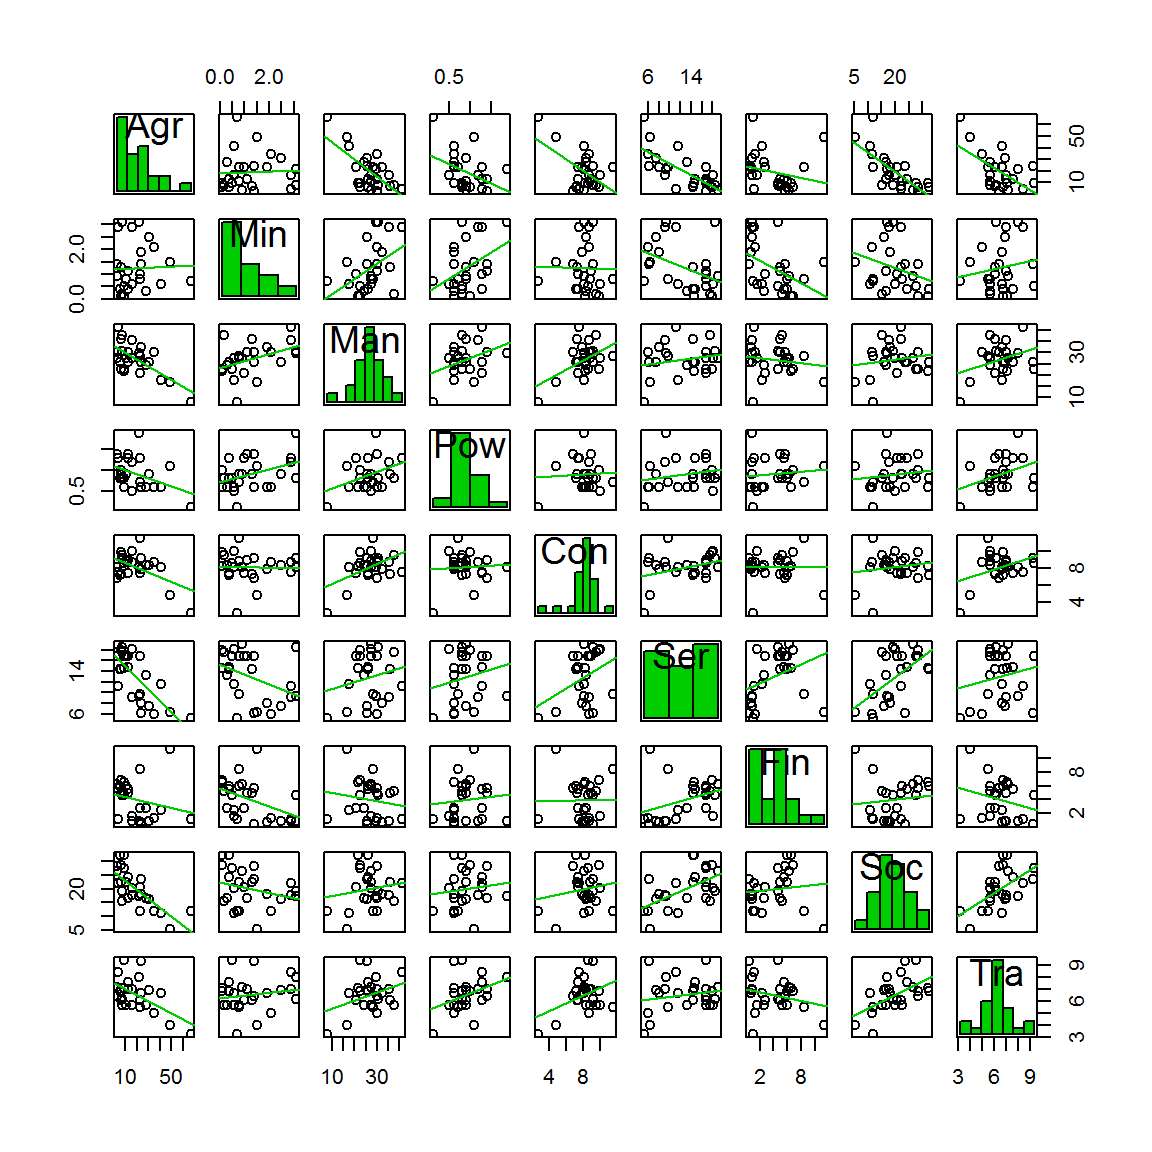
\includegraphics[width=0.7\linewidth]{Machine-Learning_files/figure-latex/unnamed-chunk-9-1} \end{center}

We definitely need a way of visualizing and quantifying the relations
between variables for a moderate to large amount of variables. PCA will
be a handy way. Recall what PCA does:

\begin{enumerate}
\def\labelenumi{\arabic{enumi}.}
\tightlist
\item
  Takes the data for the variables \(X_1,\ldots,X_p\).
\item
  Using this data, looks for new variables
  \(\text{PC}_1,\ldots \text{PC}_p\) such that:

  \begin{itemize}
  \tightlist
  \item
    \(\text{PC}_j\) is a \textbf{linear combination} of
    \(X_1,\ldots,X_k\), \(1\leq j\leq p\). This is,
    \(\text{PC}_j=a_{1j}X_1+a_{2j}X_2+\ldots+a_{pj}X_p\).
  \item
    \(\text{PC}_1,\ldots \text{PC}_p\) are \textbf{sorted decreasingly
    in terms of variance}. Hence \(\text{PC}_j\) has more variance than
    \(\text{PC}_{j+1}\), \(1\leq j\leq p-1\),
  \item
    \(\text{PC}_{j_1}\) and \(\text{PC}_{j_2}\) are
    \textbf{uncorrelated}, for \(j_1\neq j_2\).
  \item
    \(\text{PC}_1,\ldots \text{PC}_p\) have the \textbf{same
    information}, measured in terms of \textbf{total variance}, as
    \(X_1,\ldots,X_p\).
  \end{itemize}
\item
  Produces three key objects:

  \begin{itemize}
  \tightlist
  \item
    \textbf{Variances of the PCs}. They are sorted decreasingly and give
    an idea of which PCs are contain most of the information of the data
    (the ones with more variance).
  \item
    \textbf{Weights of the variables in the PCs}. They give the
    interpretation of the PCs in terms of the original variables, as
    they are the coefficients of the linear combination. The weights of
    the variables \(X_1,\ldots,X_p\) on the PC\(_j\),
    \(a_{1j},\ldots,a_{pj}\), are normalized:
    \(a_{1j}^2+\ldots+a_{pj}^2=1\), \(j=1,\ldots,p\). In \texttt{R},
    they are called \texttt{loadings}.
  \item
    \textbf{Scores of the data in the PCs}: this is the data with
    \(\text{PC}_1,\ldots \text{PC}_p\) variables instead of
    \(X_1,\ldots,X_p\). The \textbf{scores are uncorrelated}. Useful for
    knowing which PCs have more effect on a certain observation.
  \end{itemize}
\end{enumerate}

Hence, PCA rearranges our variables in an information-equivalent, but
more convenient, layout where the variables are \textbf{sorted according
to the ammount of information they are able to explain}. From this
position, the next step is clear: \textbf{stick only with a limited
number of PCs such that they explain most of the information} (e.g.,
70\% of the total variance) and do \emph{dimension reduction}. The
effectiveness of PCA in practice varies from the structure present in
the dataset. For example, in the case of highly dependent data, it could
explain more than the 90\% of variability of a dataset with tens of
variables with just two PCs.

Let's see how to compute a full PCA in \texttt{R}.

\begin{Shaded}
\begin{Highlighting}[]
\CommentTok{# The main function - use cor = TRUE to avoid scale distortions}
\NormalTok{pca <-}\StringTok{ }\KeywordTok{princomp}\NormalTok{(eurojob, }\DataTypeTok{cor =} \OtherTok{TRUE}\NormalTok{)}

\CommentTok{# What is inside?}
\KeywordTok{str}\NormalTok{(pca)}
\CommentTok{#ans> List of 7}
\CommentTok{#ans>  $ sdev    : Named num [1:9] 1.867 1.46 1.048 0.997 0.737 ...}
\CommentTok{#ans>   ..- attr(*, "names")= chr [1:9] "Comp.1" "Comp.2" "Comp.3" "Comp.4" ...}
\CommentTok{#ans>  $ loadings: loadings [1:9, 1:9] -0.52379 -0.00132 0.3475 0.25572 0.32518 ...}
\CommentTok{#ans>   ..- attr(*, "dimnames")=List of 2}
\CommentTok{#ans>   .. ..$ : chr [1:9] "Agr" "Min" "Man" "Pow" ...}
\CommentTok{#ans>   .. ..$ : chr [1:9] "Comp.1" "Comp.2" "Comp.3" "Comp.4" ...}
\CommentTok{#ans>  $ center  : Named num [1:9] 19.131 1.254 27.008 0.908 8.165 ...}
\CommentTok{#ans>   ..- attr(*, "names")= chr [1:9] "Agr" "Min" "Man" "Pow" ...}
\CommentTok{#ans>  $ scale   : Named num [1:9] 15.245 0.951 6.872 0.369 1.614 ...}
\CommentTok{#ans>   ..- attr(*, "names")= chr [1:9] "Agr" "Min" "Man" "Pow" ...}
\CommentTok{#ans>  $ n.obs   : int 26}
\CommentTok{#ans>  $ scores  : num [1:26, 1:9] 1.71 0.953 0.755 0.853 -0.104 ...}
\CommentTok{#ans>   ..- attr(*, "dimnames")=List of 2}
\CommentTok{#ans>   .. ..$ : chr [1:26] "Belgium" "Denmark" "France" "WGerm" ...}
\CommentTok{#ans>   .. ..$ : chr [1:9] "Comp.1" "Comp.2" "Comp.3" "Comp.4" ...}
\CommentTok{#ans>  $ call    : language princomp(x = eurojob, cor = TRUE)}
\CommentTok{#ans>  - attr(*, "class")= chr "princomp"}

\CommentTok{# The standard deviation of each PC}
\NormalTok{pca}\OperatorTok{$}\NormalTok{sdev}
\CommentTok{#ans>  Comp.1  Comp.2  Comp.3  Comp.4  Comp.5  Comp.6  Comp.7  Comp.8  Comp.9 }
\CommentTok{#ans> 1.86739 1.45951 1.04831 0.99724 0.73703 0.61922 0.47514 0.36985 0.00675}

\CommentTok{# Weights: the expression of the original variables in the PCs}
\CommentTok{# E.g. Agr = -0.524 * PC1 + 0.213 * PC5 - 0.152 * PC6 + 0.806 * PC9}
\CommentTok{# And also: PC1 = -0.524 * Agr + 0.347 * Man + 0256 * Pow + 0.325 * Con + ...}
\CommentTok{# (Because the matrix is orthogonal, so the transpose is the inverse)}
\NormalTok{pca}\OperatorTok{$}\NormalTok{loadings}
\CommentTok{#ans> }
\CommentTok{#ans> Loadings:}
\CommentTok{#ans>     Comp.1 Comp.2 Comp.3 Comp.4 Comp.5 Comp.6 Comp.7 Comp.8 Comp.9}
\CommentTok{#ans> Agr -0.524                       0.213 -0.153                0.806}
\CommentTok{#ans> Min        -0.618 -0.201        -0.164  0.101  0.726              }
\CommentTok{#ans> Man  0.347 -0.355 -0.150  0.346 -0.385  0.288 -0.479  0.126  0.366}
\CommentTok{#ans> Pow  0.256 -0.261 -0.561 -0.393  0.295 -0.357 -0.256 -0.341       }
\CommentTok{#ans> Con  0.325         0.153  0.668  0.472 -0.130  0.221 -0.356       }
\CommentTok{#ans> Ser  0.379  0.350 -0.115        -0.284 -0.615  0.229  0.388  0.238}
\CommentTok{#ans> Fin         0.454 -0.587         0.280  0.526  0.187  0.174  0.145}
\CommentTok{#ans> Soc  0.387  0.222  0.312 -0.412 -0.220  0.263  0.191 -0.506  0.351}
\CommentTok{#ans> Tra  0.367 -0.203  0.375 -0.314  0.513  0.124         0.545       }
\CommentTok{#ans> }
\CommentTok{#ans>                Comp.1 Comp.2 Comp.3 Comp.4 Comp.5 Comp.6 Comp.7 Comp.8}
\CommentTok{#ans> SS loadings     1.000  1.000  1.000  1.000  1.000  1.000  1.000  1.000}
\CommentTok{#ans> Proportion Var  0.111  0.111  0.111  0.111  0.111  0.111  0.111  0.111}
\CommentTok{#ans> Cumulative Var  0.111  0.222  0.333  0.444  0.556  0.667  0.778  0.889}
\CommentTok{#ans>                Comp.9}
\CommentTok{#ans> SS loadings     1.000}
\CommentTok{#ans> Proportion Var  0.111}
\CommentTok{#ans> Cumulative Var  1.000}

\CommentTok{# Scores of the data on the PCs: how is the data reexpressed into PCs}
\KeywordTok{head}\NormalTok{(pca}\OperatorTok{$}\NormalTok{scores, }\DecValTok{10}\NormalTok{)}
\CommentTok{#ans>         Comp.1  Comp.2  Comp.3  Comp.4  Comp.5  Comp.6  Comp.7 Comp.8}
\CommentTok{#ans> Belgium  1.710  1.2218 -0.1148 -0.3395 -0.3245  0.0473  0.3401  0.403}
\CommentTok{#ans> Denmark  0.953  2.1278  0.9507 -0.5939  0.1027  0.8273  0.3029 -0.352}
\CommentTok{#ans> France   0.755  1.1212 -0.4980  0.5003 -0.2997 -0.1158  0.1855 -0.266}
\CommentTok{#ans> WGerm    0.853  0.0114 -0.5795  0.1105 -1.1652  0.6181 -0.4446  0.194}
\CommentTok{#ans> Ireland -0.104  0.4140 -0.3840 -0.9267  0.0152 -1.4242  0.0370 -0.334}
\CommentTok{#ans> Italy    0.375  0.7695  1.0606  1.4772 -0.6452 -1.0021  0.1418 -0.130}
\CommentTok{#ans> Luxem    1.059 -0.7558 -0.6515  0.8352 -0.8659 -0.2188  1.6942  0.547}
\CommentTok{#ans> Nether   1.688  2.0048  0.0637  0.0235  0.6352 -0.2120  0.3034 -0.591}
\CommentTok{#ans> UK       1.630  0.3731 -1.1409 -1.2669 -0.8129  0.0361 -0.0413 -0.349}
\CommentTok{#ans> Austria  1.176 -0.1431 -1.0434  0.1577  0.5210 -0.8019 -0.4150  0.215}
\CommentTok{#ans>            Comp.9}
\CommentTok{#ans> Belgium -0.001090}
\CommentTok{#ans> Denmark  0.015619}
\CommentTok{#ans> France  -0.000507}
\CommentTok{#ans> WGerm   -0.006539}
\CommentTok{#ans> Ireland  0.010879}
\CommentTok{#ans> Italy    0.005602}
\CommentTok{#ans> Luxem    0.003453}
\CommentTok{#ans> Nether  -0.010931}
\CommentTok{#ans> UK      -0.005478}
\CommentTok{#ans> Austria -0.002816}

\CommentTok{# Scatterplot matrix of the scores - they are uncorrelated!}
\KeywordTok{scatterplotMatrix}\NormalTok{(pca}\OperatorTok{$}\NormalTok{scores, }\DataTypeTok{reg.line =}\NormalTok{ lm, }\DataTypeTok{smooth =} \OtherTok{FALSE}\NormalTok{, }\DataTypeTok{spread =} \OtherTok{FALSE}\NormalTok{,}
                  \DataTypeTok{span =} \FloatTok{0.5}\NormalTok{, }\DataTypeTok{ellipse =} \OtherTok{FALSE}\NormalTok{, }\DataTypeTok{levels =} \KeywordTok{c}\NormalTok{(.}\DecValTok{5}\NormalTok{, .}\DecValTok{9}\NormalTok{), }\DataTypeTok{id.n =} \DecValTok{0}\NormalTok{,}
                  \DataTypeTok{diagonal =} \StringTok{'histogram'}\NormalTok{)}
\end{Highlighting}
\end{Shaded}

\begin{center}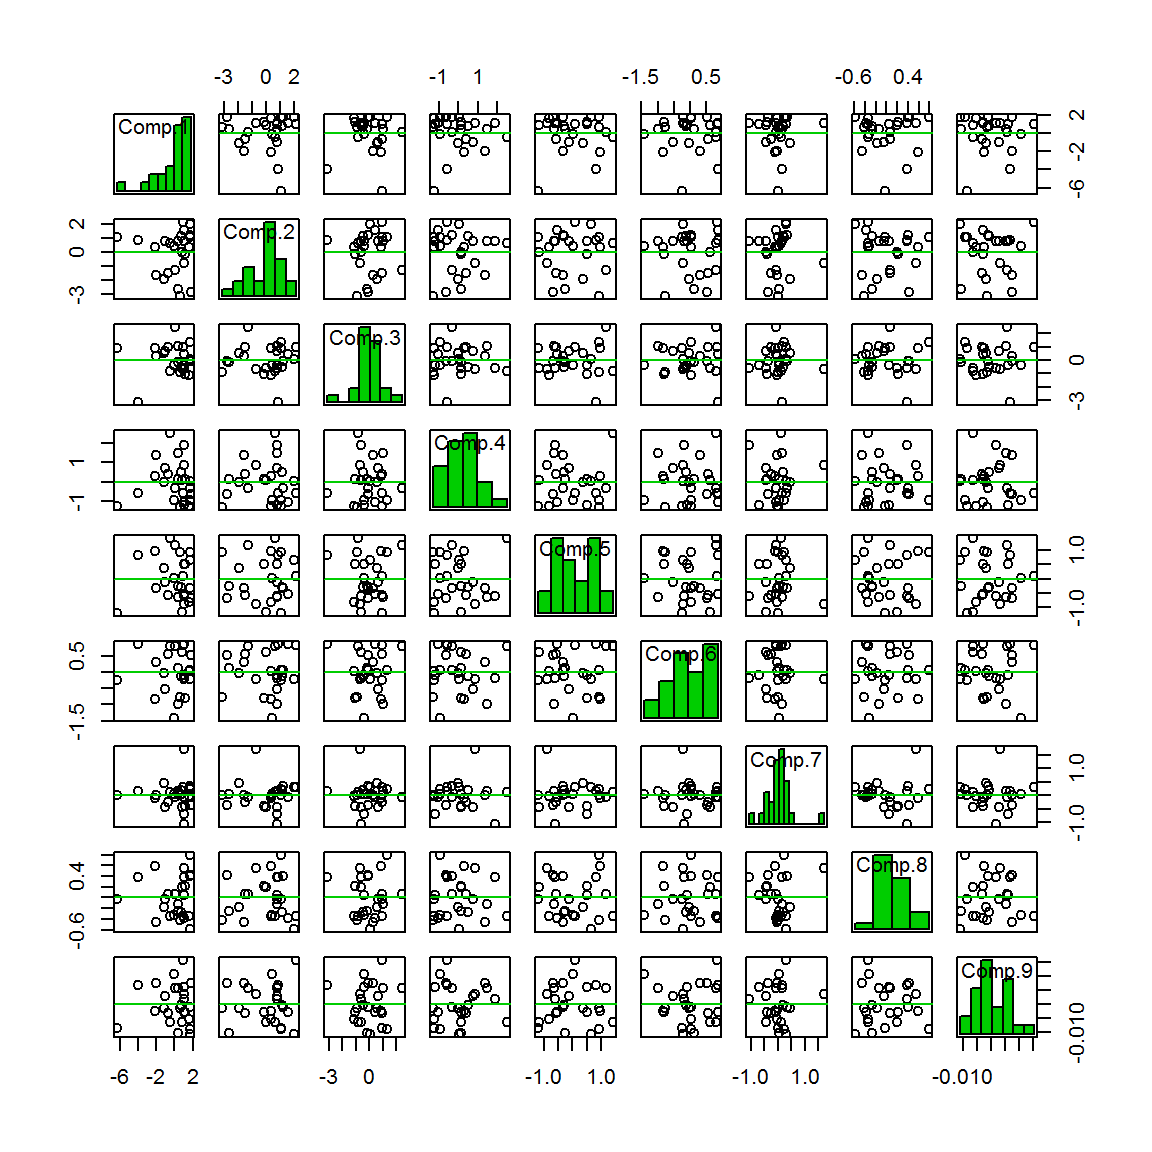
\includegraphics[width=0.7\linewidth]{Machine-Learning_files/figure-latex/unnamed-chunk-10-1} \end{center}

\begin{Shaded}
\begin{Highlighting}[]

\CommentTok{# Means of the variables - before PCA the variables are centered}
\NormalTok{pca}\OperatorTok{$}\NormalTok{center}
\CommentTok{#ans>    Agr    Min    Man    Pow    Con    Ser    Fin    Soc    Tra }
\CommentTok{#ans> 19.131  1.254 27.008  0.908  8.165 12.958  4.000 20.023  6.546}

\CommentTok{# Rescalation done to each variable}
\CommentTok{# - if cor = FALSE (default), a vector of ones}
\CommentTok{# - if cor = TRUE, a vector with the standard deviations of the variables}
\NormalTok{pca}\OperatorTok{$}\NormalTok{scale}
\CommentTok{#ans>    Agr    Min    Man    Pow    Con    Ser    Fin    Soc    Tra }
\CommentTok{#ans> 15.245  0.951  6.872  0.369  1.614  4.486  2.752  6.697  1.364}

\CommentTok{# Summary of the importance of components - the third row is key}
\KeywordTok{summary}\NormalTok{(pca)}
\CommentTok{#ans> Importance of components:}
\CommentTok{#ans>                        Comp.1 Comp.2 Comp.3 Comp.4 Comp.5 Comp.6 Comp.7}
\CommentTok{#ans> Standard deviation      1.867  1.460  1.048  0.997 0.7370 0.6192 0.4751}
\CommentTok{#ans> Proportion of Variance  0.387  0.237  0.122  0.110 0.0604 0.0426 0.0251}
\CommentTok{#ans> Cumulative Proportion   0.387  0.624  0.746  0.857 0.9171 0.9597 0.9848}
\CommentTok{#ans>                        Comp.8   Comp.9}
\CommentTok{#ans> Standard deviation     0.3699 6.75e-03}
\CommentTok{#ans> Proportion of Variance 0.0152 5.07e-06}
\CommentTok{#ans> Cumulative Proportion  1.0000 1.00e+00}

\CommentTok{# Scree plot - the variance of each component}
\KeywordTok{plot}\NormalTok{(pca)}
\end{Highlighting}
\end{Shaded}

\begin{center}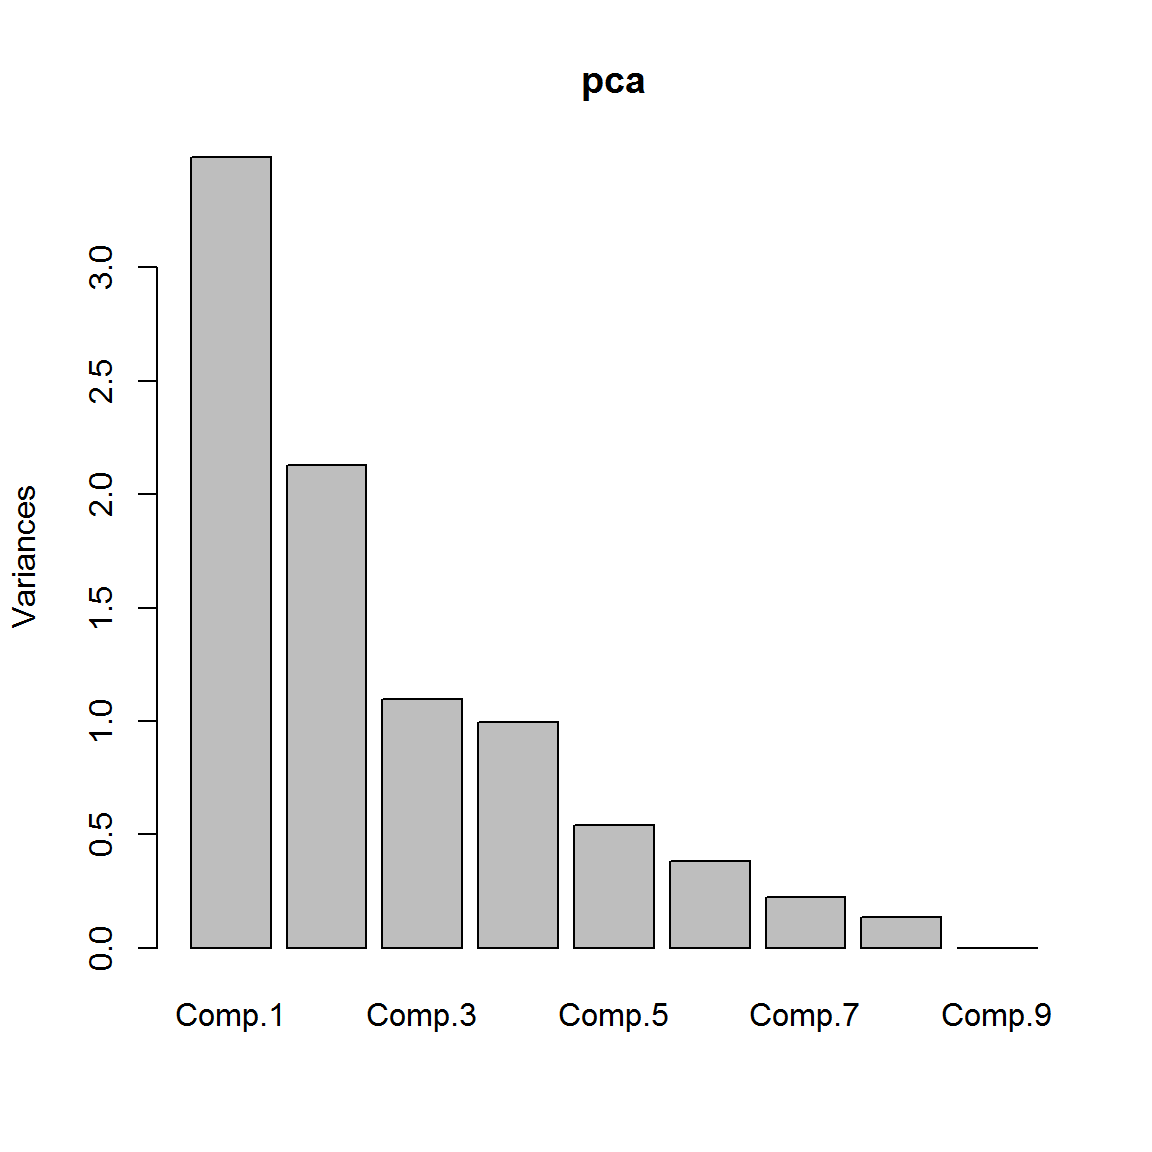
\includegraphics[width=0.7\linewidth]{Machine-Learning_files/figure-latex/unnamed-chunk-10-2} \end{center}

\begin{Shaded}
\begin{Highlighting}[]

\CommentTok{# With connected lines - useful for looking for the "elbow"}
\KeywordTok{plot}\NormalTok{(pca, }\DataTypeTok{type =} \StringTok{"l"}\NormalTok{)}
\end{Highlighting}
\end{Shaded}

\begin{center}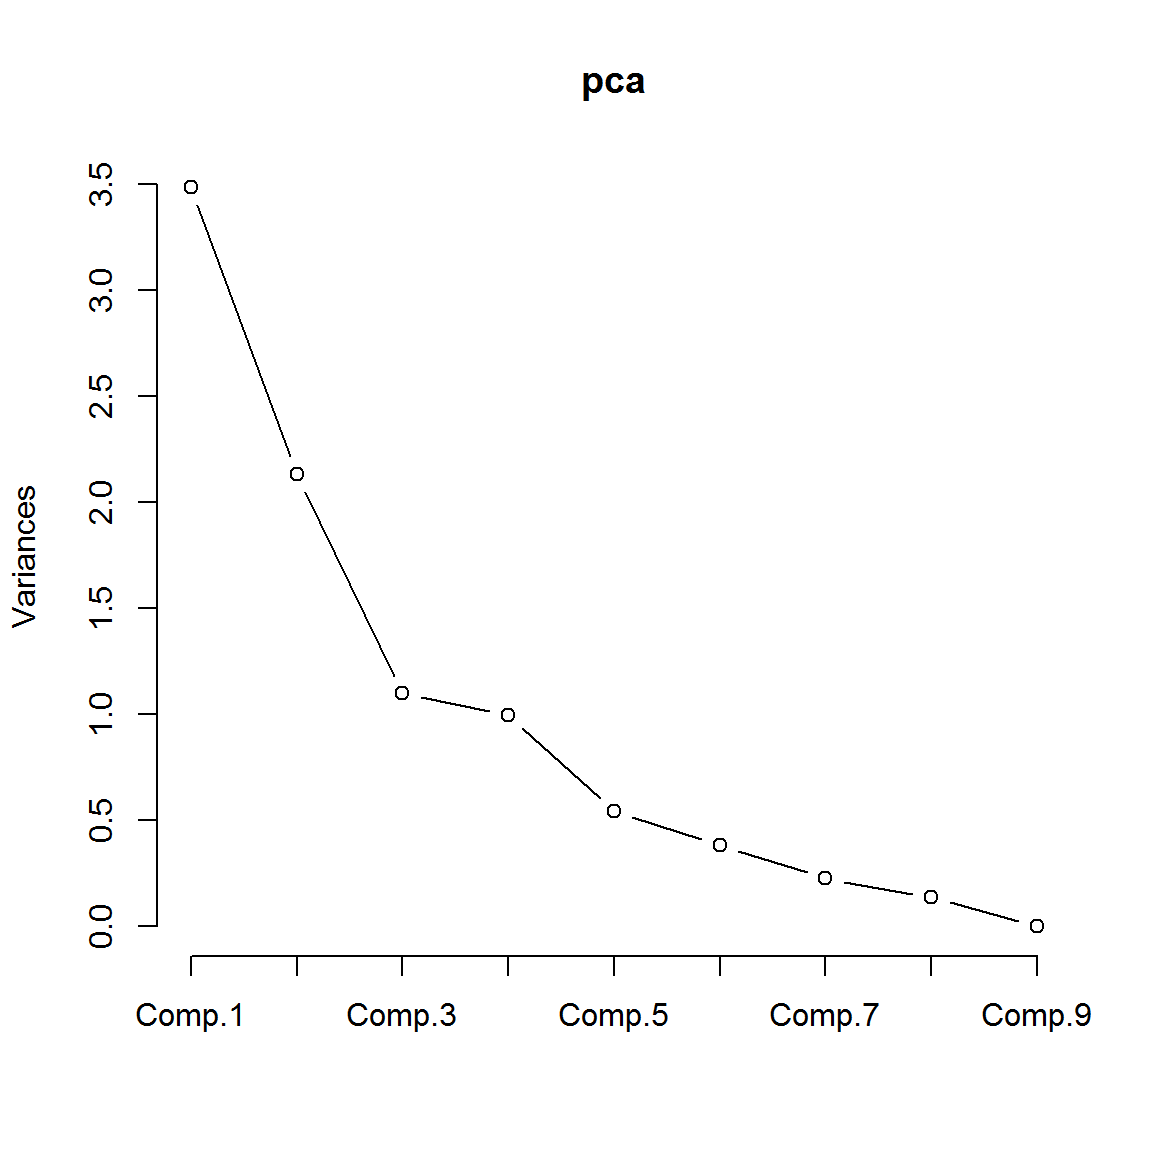
\includegraphics[width=0.7\linewidth]{Machine-Learning_files/figure-latex/unnamed-chunk-10-3} \end{center}

\begin{Shaded}
\begin{Highlighting}[]

\CommentTok{# PC1 and PC2}
\NormalTok{pca}\OperatorTok{$}\NormalTok{loadings[, }\DecValTok{1}\OperatorTok{:}\DecValTok{2}\NormalTok{]}
\CommentTok{#ans>       Comp.1  Comp.2}
\CommentTok{#ans> Agr -0.52379 -0.0536}
\CommentTok{#ans> Min -0.00132 -0.6178}
\CommentTok{#ans> Man  0.34750 -0.3551}
\CommentTok{#ans> Pow  0.25572 -0.2611}
\CommentTok{#ans> Con  0.32518 -0.0513}
\CommentTok{#ans> Ser  0.37892  0.3502}
\CommentTok{#ans> Fin  0.07437  0.4537}
\CommentTok{#ans> Soc  0.38741  0.2215}
\CommentTok{#ans> Tra  0.36682 -0.2026}
\end{Highlighting}
\end{Shaded}

\begin{rmdinsight}
PCA produces \textbf{uncorrelated} variables from the original set
\(X_1,\ldots,X_p\). This implies that:

\begin{itemize}
\tightlist
\item
  The PCs are uncorrelated, \textbf{but not independent} (uncorrelated
  does not imply independent).
\item
  An uncorrelated or independent variable in \(X_1,\ldots,X_p\) will get
  a PC only associated to it. In the extreme case where all the
  \(X_1,\ldots,X_p\) are uncorrelated, these coincide with the PCs (up
  to sign flips).
\end{itemize}
\end{rmdinsight}

Based on the weights of the variables on the PCs, we can extract the
following interpretation:

\begin{itemize}
\tightlist
\item
  PC1 is roughly a linear combination of \texttt{Agr}, with
  \emph{negative} weight, and (\texttt{Man}, \texttt{Pow}, \texttt{Con},
  \texttt{Ser}, \texttt{Soc}, \texttt{Tra}), with \emph{positive}
  weights. So it can be interpreted as an \emph{indicator} of the kind
  of economy of the country: agricultural (negative values) or
  industrial (positive values).
\item
  PC2 has \emph{negative} weights on (\texttt{Min}, \texttt{Man},
  \texttt{Pow}, \texttt{Tra}) and \emph{positive} weights in
  (\texttt{Ser}, \texttt{Fin}, \texttt{Soc}). It can be interpreted as
  the contrast between relatively large or small service sectors. So it
  tends to be negative in communist countries and positive in capitalist
  countries.
\end{itemize}

\begin{rmdtip}
The interpretation of the PCs involves inspecting the weights and
interpreting the linear combination of the original variables, which
might be separating between two clear characteristics of the data
\end{rmdtip}

To conclude, let's see how we can represent our original data into a
plot called \emph{biplot} that summarizes all the analysis for two PCs.

\begin{Shaded}
\begin{Highlighting}[]
\CommentTok{# Biplot - plot together the scores for PC1 and PC2 and the}
\CommentTok{# variables expressed in terms of PC1 and PC2}
\KeywordTok{biplot}\NormalTok{(pca)}
\end{Highlighting}
\end{Shaded}

\begin{center}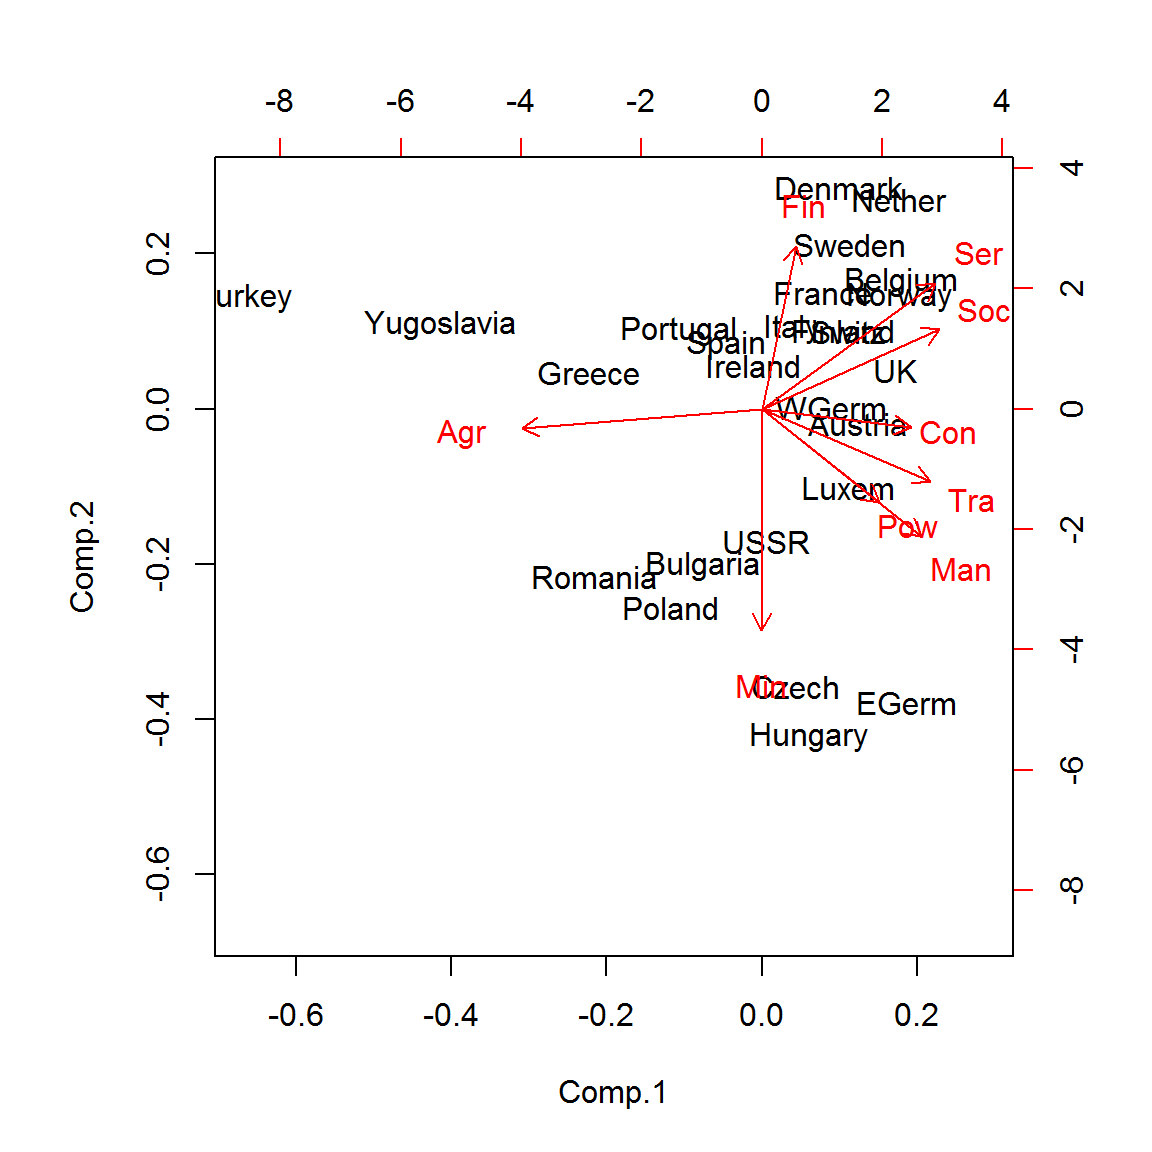
\includegraphics[width=0.9\linewidth]{Machine-Learning_files/figure-latex/unnamed-chunk-13-1} \end{center}

◼


\end{document}
